\graphicspath{ {img/Survey/} }
\chapter[Automated Spectrum Trading Mechanisms: Understanding the Big Picture][Automated Spectrum Trading Mechanisms]{Automated Spectrum Trading Mechanisms: Understanding the Big Picture}\label{Survey_chap}
\section{Introduction}\label{Survey_sec_Intro}
In this second part of the thesis, we focus on automated spectrum trading mechanisms.
Compared to other DSA approaches, automated spectrum trading has the advantage of providing economic (and/or other) incentives to the entities involved, especially important to licensed operators, encouraging the adoption of DSA and promoting motivation for future investments in primary spectrum acquisitions.
Nevertheless, deploying a secondary spectrum trading market could also cause the opposite result if is not properly crafted, that is, undermining the competition structure, by giving rise to collusive behaviors and/or service providers becoming monopolists (see the introduction of Sect. \ref{subsec:Oligo} of this chapter and \cite{ref:Yoon2012}, especially its Sect. 5.2 \enquote{Comparison of competition: tipping effects}).

This chapter contains a comprehensive survey on automated spectrum trading which, to the best of our knowledge, is novel in its treatment of the subject in the following key aspects: its scope (a general view of spectrum trading), the proposed classification of the different issues and approaches in spectrum trading, its tutorial nature, its coverage of the most up-to-date works, and the identification of the main open problems.  

\subsection{Motivation of Automated Spectrum Trading}
Previous works in economic theory are not easily translated to spectrum trading because of the specific features of the traded good. A spectrum market poses the following additional challenges:
\begin{itemize}
\tightlist
\item{Rapid variations with time}
\item{Imperfect information}
\item{Complex resource allocation considering re-utilization and heterogeneity of the good}
\end{itemize}

Both spectrum supply and demand changes are related to data traffic intensity which, in general, experiences \textit{rapid variations with time}. 
In addition, spectrum characteristics are also highly variable, in particular, availability and channel quality parameters. If trading decisions could be made in such short time-scales (possibly in the order of seconds), the spectrum exploitation efficiency would increase. This implies that the agents making the decisions in the spectrum markets have to be computerized. Automatic transactions are present in financial trading (\cite{ref:Adler2012}), but that market does not show the specific issues of spectrum trading. 

\textit{Imperfect information} not only refers to the competitive behavior of agents in a traditional market, by which they are not willing to reveal their true valuation of a good. 
It also refers to the fact that agents may not have complete or reliable information about the market due to the communication complexity that it would involve, specially in ad-hoc networks. 
It entails unfeasible requirements such as, for example, all entities knowing all channel gains between each other.

\textit{Resource allocation} becomes more complicated with spectrum as a traded good because, depending on the mutual interference ranges of the entities, it can be \textit{spatially reused}. 
It may also be considered that spectrum is an \textit{heterogeneous} good, in the sense that the same spectrum portion can be valuated differently by each user, depending on its position, technology (spectrum efficiency use), etc. 

Rapid variations with time and resource allocation in complex models are tightly interrelated.
Optimal resource allocation in complex models requires a computational time that makes it hard to keep up with the rapid changes, which, in turn, may render a solution inefficient because of a time dis-adaptation. 
Dealing with imperfect information makes optimal resource allocation more complex, even intractable. On the contrary, local estimations could be considered, sacrificing model optimality for the sake of speed.

\subsection{Our Contribution}
\newcolumntype{x}[1]{>{\centering\let\newline\\\arraybackslash\hspace{0pt}}p{#1}}
Our contribution in this chapter is summarized as follows:
\begin{itemize}
\tightlist
\item Our work is unique in its scope, focusing on automated spectrum trading as the most promising mechanism to solve spectrum scarcity.
\item We identify the specific aspects that make spectrum different from conventional goods and the impact that these features have on automatic trading.
\item We discuss past and current approaches, as well as future research lines, highlighting their advantages and disadvantages. 
\item Each sub-topic is presented and developed explicitly with references to previous works where each aspect has been considered or addressed.
\item This work can serve as an introduction to the field for novel researchers, and is useful to experienced ones for its critical discussion of the most recent trends.
\item Finally, as a conclusion of the surveying effort, we highlight overlooked issues of automated spectrum trading, with a special focus on practical implementation.
\end{itemize}

Compared to previous works in this area such as \cite{ref:Maharjan2011,ref:Niyato2008_Spec,ref:Hossain2009,ref:Huang2013,ref:Zhang2013,ref:Akkara2011,ref:Zhang2012}, our work covers a broader range of aspects, as summarized in Table \ref{survey_table_related_work}.
Although the scope of \cite{ref:Maharjan2011} claims to be ``economic approaches'', it devotes part of the survey to dynamic spectrum access, which has its own particularities. 
In addition, it is structured around a classification of related works where the items are a mix of mathematical tools and market principles, specially focusing on game theory, while our work extends the classification including further aspects in spectrum trading such as its objectives, mechanisms, possible market forms, etc. 
We also perform a deeper identification of key issues in the entities' decision, especially real-time adaptation, which could be considered as one of the most critical aspects for a spectrum trading mechanism to achieve an efficient solution. 
There is a small essay on spectrum sharing and trading in \cite{ref:Niyato2008_Spec}, and \cite{ref:Hossain2009} presents a general study of spectrum trading with a notable tutorial approach. 
Compared to these works, our survey offers an extensive coverage of the advances in this field during the last five years, showing an upgraded taxonomy comprising the most novel proposals. 
From a different perspective other works cover only part of the issues addressed in this survey: \cite{ref:Huang2013} is a survey of spectrum trading for Cooperative Secondary Spectrum Access (CSSA) under imperfect information, \cite{ref:Zhang2013} is concerned with self-organization paradigms in cognitive radio and \cite{ref:Akkara2011,ref:Zhang2012} develop a summary of game theoretic and auction approaches in dynamic spectrum access respectively. 

The rest of this chapter is organized as follows. In section \ref{sec:Trading} we show key points in the spectrum trading mechanism design. Section \ref{sec:TradedGood} reviews the challenges arising as a consequence of the special properties of spectrum as a trading good. The mathematical tools used to study these trading models are discussed in section \ref{sec:Math}. How those techniques are used in different market forms is analyzed in section \ref{sec:Market}. Finally, we provide some guidelines and feedback for future research in section \ref{sec:Open} and summarize the main conclusions of this survey in section \ref{sec:Conclusions}.

\begin{landscape}
\begin{table*}
\setlength{\tabcolsep}{3pt}
\scriptsize
\caption{Summary of related works.''E'' means the topic is developed explicitly, ``I'' means the topic is developed implicitly, ``M'' means the topic is mentioned but not developed, ``X'' means the topic is not present. }
\label{survey_table_related_work}
\rowcolors{6}{}{lightgray}
\begin{tabular}{p{4.5cm}lllllllll|}
\hline
&	\textbf{Our work} 			& \cite{ref:Maharjan2011} & \cite{ref:Niyato2008_Spec} 		& \cite{ref:Hossain2009} & \cite{ref:Huang2013} & \cite{ref:Zhang2013} 	& \cite{ref:Akkara2011} & \cite{ref:Zhang2012} \\

Scope																		& Spec. trading & DSA and spec. trading 	& DSA and spec. trading 				& DSA 									 & CSSA in imperfect info. & Self-org.	& Game Th. DSA  				& Spec. auctions \\
Type of work														& Survey 				& Survey 							 		& Model												  & Book					 				 & Survey 								 & Survey							& Survey 								& Survey \\
Year																		&	2013 					& 2010 										& 2008 													& 2008 									 & 2013 									 & 2013 							& 2011 									& 2012 \\
Number of references										&	98	 					& 36 											& 14 														& \textless 30 									 & 15 										 & 15 								& 74 										& 32 \\
\hline
Economic objectives											&	\textbf{E} 		& X												& X 														& I 										 & X 											 & X 									& \textbf{E} 						& \textbf{E} \\ 

CSSA																		&	\textbf{E} 		& X 											& X 														& \textbf{E} 						 & \textbf{E} 						 & \textbf{E} 				& M 										& M \\

Real-time variations										&	\textbf{E} 		& X 											& X 														& X 										 & X											 & I 									& I 										& M \\

Imperfect information										&	\textbf{E} 		& I 											& M 														& \textbf{E} 						 & \textbf{E}							 & I 									& \textbf{E} 						& M \\

Spatial reuse														&	\textbf{E} 		& X 											& X 														& X 										 & M											 & X 									& X 										& \textbf{E} \\

Heterogeneity														&	\textbf{E} 		& M 											& X 														& M 										 & X											 & I 									& M 										& M \\

Formulation frameworks									&	\textbf{E}	  & \textbf{E}							& \textbf{E} 									  & \textbf{E} 						 & \textbf{E}							 & M 									& \textbf{E} 						& M \\

Market forms														&	\textbf{E} 		& \textbf{E} 							& \textbf{E} 										& \textbf{E} 						 & X											 & X 									& X 										& M \\

Implementation issues										&	\textbf{E} 		& M 											& M 														& \textbf{E} 						 & \textbf{E}							 & \textbf{E} 				& I 										& \textbf{E} \\

Protection against malfunctions					&	\textbf{E} 		& \textbf{E} 							& X 														& \textbf{E} 						 & X											 & X 									& \textbf{E} 						& \textbf{E} \\
\hline				
\end{tabular}
\end{table*}
\end{landscape}

\section{Trading Mechanism Design} 
\label{sec:Trading}
\subsection{Basics} 
\label{subsec:When}
The most basic form of spectrum trading (and any trading in general) is found when the transaction takes place between just two entities. Usually one of these entities, the ``seller'', offers its unused spectrum opportunities to interested users, ``buyers'', in exchange for something (usually money). Although this situation may appear as simplistic, it is useful as more than a didactic example, since it corresponds to a real scenario in which there is only one primary and one secondary network, both with a centralized structure so the transaction is negotiated between their base stations as in Fig. \ref{fig:BasicMarket}, and, in fact, some authors have studied this market form as explained later in Section \ref{subsec:marketeq}). 

\begin{figure}[!ht]
  \begin{center}
  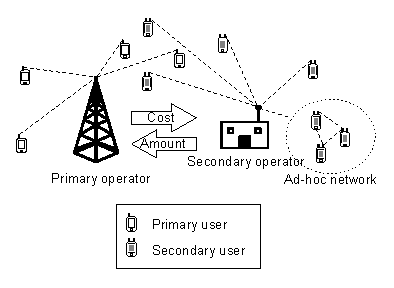
\includegraphics[scale=1.25]{Fig1.eps}
  \end{center}
  \caption{Basic spectrum trading}
   \label{fig:BasicMarket}
\end{figure}

For the buyer, the trade-off between its interest in what the seller offers and its cost is expressed by the utility function $u_i(x)$, where $x$ is an n-tuple comprising the conditions of the trade, \textit{e.g.,} the amount of spectrum bought and the price paid. Similarly, the seller is also in a compromise between the revenue it obtains from the buyer and the costs associated with the sale: interferences, higher blocking probability (because it would have less available spectrum) and fixed costs because of the investment in infrastructure. This trade-off is expressed by the profit function $\pi_i(y)$, where $y$ denotes the conditions of the trade. It can also be called utility function. Both functions return unidimensional values:
\begin{equation}
\begin {array} {lcl}
u_i, \pi_i :  \mathbb{R}^N \rightarrow \mathbb{R}
\end{array}
\end{equation}

An example of a simple utility function for buyer $i$, where bandwidth is the traded good, has the following form:
\begin{equation}
u_{i}(b_{i}, c_{i}) = k_{i}b_{i}-c_{i}b_{i}
\end{equation}
where $b_{i}$ is the amount of commodity to buy (bandwidth), $c_i$ is its cost per unit for buyer $i$ (it may not be the same for every buyer) and $k_{i}$ characterizes the value given by the SU to the spectrum units. The valuation of the bandwidth is then $k_{i}b_{i}$, while $c_{i}b_{i}$ represents the cost. It is far from trivial to select which metrics should be combined in a utility/profit function to quantify the impact of spectrum trading on each agent's outcome, and which constraints should be imposed. The metric used strongly influences the outcome of the trading models \cite{ref:YZhao2009}. One usual approach is to use logarithmic functions to model the ``law of diminishing returns'': if the obtained resource is increased, at some point satisfaction will saturate because no more resources are really needed.

When there are multiple sellers and buyers in an area,  the conflict between sellers and buyers gets more complex because of the added interactions brought by competition among sellers. The price per unit of a seller depends on the price per unit of the other sellers, as rational buyers will buy from the cheapest. There is also competition among buyers for the finite resource or in terms of mutual interferences and price charged depending on their total aggregate demand. The key of a spectrum trading mechanism design is to obtain policies for the entities involved so that they agree in the amount of commodity to be sold (supply) and bought (demand) as well as its price, in order to reach some particular objective. 

\subsection{Economic Objectives}
\label{subsec:Objective}	

\begin{table}
\rowcolors{1}{}{lightgray}
\caption{Classification of different works by their economic objective}
\label{Survey_table_economic_obj}
\begin{tabular}{lL{8cm}} 
\hline
\textbf{Main economic objective} & \textbf{Works} \\
\hline
Benefit of the spectrum owner & \cite{ref:Mutlu2008,ref:Yu2010,ref:Gao2011,ref:Yang2011,ref:Simeone2008,ref:Zhang2009,ref:Yi2010,ref:Li2011,ref:Duan2011_Contract,ref:Jayaweera2009,ref:Jayaweera2010,ref:Vazquez2010,ref:Maille2009,ref:Guijarro2011,ref:Niyato2008_Comp,ref:Dixit2010,ref:Sengupta2007,ref:Sengupta2009,ref:Jia2009_Rev,ref:Kaskebar2012} \\
Social optimum & \cite{ref:Wang2008,ref:Huang2006,ref:Huang2008_auc,ref:Gopinathan2011,ref:Xu2011,ref:Ji2008,ref:Zhu2012,ref:Niyato2007_Hier,ref:Niyato2007_Eq,ref:Niyato2008_Mark,ref:Niyato2008_Spec,ref:Niyato2010,ref:Zhou2009_TRUST,ref:Wang2010_TODA,ref:Wang2010_Spec,ref:Gao2011_MAP,ref:Xu2010,ref:Xu2012}\\
Benefit of intermediaries & \cite{ref:Illeri2005,ref:Duan2010_Cog,ref:Jia2008_com,ref:Xing2007,ref:Duan2010_Comp,ref:Duan2011_Duo,ref:Duan2011_Inves,ref:Min2011,ref:Kim2011,ref:Sengupta2007,ref:Sengupta2009,ref:Zhu2012_Dyn,ref:Min2011}\\\hline
\end{tabular}
\end{table}

In the introduction of this thesis, we explained that spectrum is scarce because it has been assigned inefficiently.
Accordingly, every automated spectrum trading system tries to improve that efficiency, but who should benefit the most from that improvement? Politics aside, the first answer that may come to our minds would be ``those who need it the most'', that is to say, \textit{maximizing the social welfare}. Even if we think it is the only possible answer, we still have to consider a fact about motivation: in order for the system to be feasible, all entities need to have an incentive to participate. In other words, no matter what the objective to maximize is, the utility functions of all the other entities need to be taken into account and be better than without the trading system (otherwise, they will not participate). And furthermore, there is one group of entities, the licensed spectrum owners, whose motivation to take part in the trading system is crucial. Then, trading mechanisms may focus on one of these other related economic objectives: \textit{maximizing the profit of the licensed spectrum } and \textit{maximizing the profit of a secondary spectrum provider}.

\begin{itemize}
\item \textit{Maximizing the social welfare.} It means maximizing an aggregate utility comprising the benefit perceived by both the spectrum owners and the unlicensed users. It is worth noting that if we do not say anything else, the concept does not include any sense of fairness. It just increases the sum of the utilities but that does not imply an equal contribution from each. That clearly has an effect on the motivation of the entities and it has been studied by multiple works like \cite{ref:Zhang2012_Fair,ref:Vidal2013,ref:Gopinathan2011,ref:Yu2010}. Social welfare with a fairness consideration could be seen as optimizing the usage of spectrum for the benefit of the whole community and therefore, it would be the objective to be pursued by the regulator authorities. This objective should be carefully balanced with the next one.  
\item \textit{Maximizing the benefit of the licensed spectrum owner.} ``Benefit'' in the sense of the utility function we shown in the previous subsection: as the combined positive and negative effects of their sale, in a variety of forms and constraints. As explained in the introduction, any form of spectrum sharing may affect licensed operators and even if that does not occur, they will be willing to receive a compensation in order to allow coexistence. Their cooperation will be boosted if they receive a proper incentive.  
\item \textit{Maximizing the benefit of a secondary spectrum provider}. A secondary spectrum provider is an entity that buys spectrum from a primary licensed owner and sells it to unlicensed users (similar to a virtual operator renting a cellular access network). This objective could be considered a particular way to give incentives to primary operators (POs). As primary operators would be able to sell their unused spectrum to these entities, they would be less reluctant to make investments in spectrum. The risk they incur is lower. In addition, changes in spectrum ownership would be more dynamic and the ability to match demands of it would increase, as these secondary operators (SOs) could focus on making direct transactions and would not go through the process of asking for long-term licenses

\end{itemize}

There are few works whose objective is maximizing the benefit of the unlicensed users (\cite{ref:Niyato2007_Game,ref:Illeri2005,ref:Niyato2009_Dyn} to cite some) and thus it has not been included as a main objective in the previous list. It would go against the idea of giving an extra incentive to primary operators. Again, we would like to remark that this does not mean that their benefit has not been taken into account: every model still aims to be incentive-compatible for every entity involved and thus, secondary utilities are also considered. There are also other approaches that do not fit exactly in any of the previous categories such as \cite{ref:Illeri2005,ref:Zhou2008}, which leave the door open to use any optimization criteria from above. Table \ref{Survey_table_economic_obj} provides a classification of different previous works by their economic objective.



\subsection{What Goods Can Be Traded}
\label{subsec:What}
\textbf{On the side of the spectrum owner}, the offered good consists of spectrum opportunities. These opportunities can be
\begin{itemize}
\item Frequency bandwidth (FDMA-like Medium Access Control [MAC]) \cite{ref:Niyato2007_Game,ref:Niyato2008_Comp,ref:Duan2010_Cog,ref:Duan2010_Comp,ref:Zhu2012_Dyn,ref:Xu2010,ref:Sengupta2007,ref:Sengupta2009,ref:Niyato2008_Mark,ref:Niyato2010,ref:Wang2010_Spec}. 
\item Power (CDMA) \cite{ref:Wang2008,ref:Yu2010,ref:Gao2011,ref:Huang2006,ref:Jayaweera2009,ref:Jayaweera2010,ref:Vazquez2010}.
\item Time\footnote{Most papers outside this category also consider the time dimension, since channels are not leased forever. However, the difference is that they consider a fixed amount of time and do not charge a price per timeshare unit.} (TDMA)  \cite{ref:Xu2011,ref:Simeone2008,ref:Zhang2009,ref:Li2011,ref:Duan2011_Contract,ref:Niyato2007_Eq}.
\item Transmission rate or capacity \cite{ref:Illeri2005,ref:Jia2008_com,ref:Maille2009} .
\item Admission to the system \cite{ref:Kaskebar2012,ref:Mutlu2008,ref:Yang2011}.
\item A combination of previous resources (referred to as ``channels'' without specification) \cite{ref:Xu2012,ref:Zhou2008,ref:Zhu2012,ref:Xing2007,ref:Jia2009_Rev,ref:Niyato2009_Dyn,ref:Niyato2007_Hier,ref:Gao2011_MAP,ref:Zhou2009_TRUST}. 
\end{itemize}

Although most of the models are flexible to use any of these ways of considering spectrum opportunities, they may influence the formulation of utility/profit functions (\textit{e.g.,} if power is being traded, the impact of channel gains on the utility/profit functions may be higher)

\textbf{On the side of the spectrum buyer}, spectrum is typically traded for money, but not always. There is a current trend in the design of trading mechanisms that considers the possibility of SUs offering their cooperation to the spectrum owner, increasing the coverage, the battery life and/or the throughput of the licensed network. This increasingly popular approach is known as \textit{Cooperative Secondary Spectrum Access} (CSSA). It also receives the names of \textit{Cooperative Spectrum Sharing} (CSS) or \textit{Cooperative Cognitive Radio Networks} (CCRNs) \cite{ref:Simeone2008,ref:Zhang2009,ref:Yi2010,ref:Vazquez2010,ref:Li2011,ref:Duan2011_Contract,ref:Duan2014,ref:Yan2013,ref:Feng2014,ref:Canzian2013}.

The premise is simple: a primary user will lease some transmission opportunities if the SUs, in exchange, act as transmission relays for the primary nodes. This is different from other market-driven spectrum sharing approaches in that it fosters the creation of transmission opportunities in the PU spectrum in an exogenous way: by increasing the transmission rate of the PU, it reduces its spectrum usage. Because of that, CSSA is particularly useful when the PU own demands are so high that it rarely has spectrum to lease.

One of the earlier proposals \cite{ref:Simeone2008}, considers one primary transmitter and receiver, and the transmission time is divided into blocks, each block containing three stages. In the first stage, the PU communicates with its intended receiver via direct link and SUs also receive the information (broadcast). On the second stage, some SUs re-transmit the same information to the primary receiver. Finally, the secondary transmitters can communicate with their intended secondary receivers. Before each transmission block, the PU tries to optimize its profit function by selecting which SUs it is willing to use as relays and determining a time assignment for each stage based on knowledge about what SUs will do (``best response'') depending on the system status (\textit{e.g.,} channel gains). After the PU makes its decision public, the selected SUs try to maximize their utilities taking into account that they will use the same amount of power for cooperating with the PU as for their own transmission. That election includes the possibility of not transmitting at all in case the bandwidth offered by the PU is not worth acting as relay. That decision is modeled with a non-cooperative power control game.

Given that framework, in \cite{ref:Zhang2009} the authors propose the consideration that a PU has certain traffic demand and once it is satisfied, it will have no incentive in improving its transmission rate and therefore it will not be willing to allow SUs to access its spectrum. In order to avoid that situation, the authors propose that SUs should also pay some monetary value to the primary. They also consider a different MAC for SUs, TDMA, rather than power control, claiming that simultaneous transmission of all SUs on an interference channel, as in \cite{ref:Simeone2008}, is unrealistic because a SNR constraint cannot be met. In \cite{ref:Zhang2009}  SUs' interactions are modeled with a non cooperative payment selection game: they have to decide how much they are willing to pay and transmission time is assigned proportionally to the amount each secondary paid with respect to the total paid by all users. Two later works \cite{ref:Yi2010,ref:Li2011}, consider more than one primary and secondary links. 
In the first one, \cite{ref:Yi2010}, the framework is extended to consider a primary and a secondary networks, both centralized. This implies that there are more than one primary transmitter-receiver pair and optimal selection of relays needs to be considered. On the other hand, SUs no longer compete as the central SUs' infrastructure takes into account aggregated utility, and thus, the payment mechanism changes. 
However, the proposal in \cite{ref:Li2011}, does the opposite, and assumes multiple selfish entities with no central authority. In addition, the authors use a different technique, coalitional games, where POs form cooperating coalitions with SUs, either involving a payment mechanism or no monetary exchange at all. A different mathematical approach is proposed in \cite{ref:Duan2011_Contract} and \cite{ref:Duan2014}, which apply the idea of contract-based trading and study different cases of incomplete information: the authors consider different types of SUs, according to their willingness to pay and their link qualities with PU receivers. An optimal contract between the PU and each SU type comprises the SU transmission powers (for PU and SU data), and the time allocated for the SU own data transmission. The contracts are designed such that each type of user will choose the contract that is designed for its type while maximizing the PU's utility. CSSA under incomplete information is also addressed by the latest works \cite{ref:Yan2013,ref:Feng2014}, applying bargaining and an auction-like mechanism, both with learning algorithms. A recent survey on the topic can be found in \cite{ref:Huang2013}.

Other related works explore alternative flavors of CSSA. For example, paper \cite{ref:Canzian2013} develops a model in which the collaborating SUs are rewarded in the time domain, with increased access opportunities to a base station (or access node), instead of bandwidth; \cite{ref:Tran2014} explores the possibility of both PUs and SUs acting as relays of each other assuming a cooperative attitude between them; and \cite{ref:Shao2014} shows the optimal strategy of a SU which is allowed to dynamically decide whether it enters a CSSA or a spectrum leasing market. 

A close related topic to CSSA is the \textit{overlay} cognitive radio network paradigm \cite{ref:Goldsmith2009}, by which a SU acts as relay for the PU and, at the same time, transmits its own message. The interference constraint on the SU transmission is enlarged thanks to the cooperative transmission and the use of interference cancellation techniques \cite{ref:Han2010}. 

\subsection{Market Mechanisms}
\label{subsec:Market}
As we showed earlier, buyers and sellers have conflicting objectives. They have to agree on the conditions of the trade, mainly amount of the traded good and its price, but they can also negotiate its quality, whether it is a temporal or a permanent lease of its exploitation rights, etc. Their negotiation process follows one of the following general mechanisms: \textit{pricing, auction} or \textit{bargaining}. 
	
\subsubsection{Pricing}
Initially, it was the most common mechanism in spectrum trading works. The sellers compute their offers and announce them. Buyers choose whether to connect with the one they are most interested in or not to establish any connection. It is almost like a ``supermarket of spectrum'' but with the associated peculiarities described when discussing spectrum as a traded good. 

In order to find the optimal price that would maximize the seller's utility function (profit), the seller would need to know information such as the demand function of the buyers or the existence and strategy of other buyers. Early research in pricing assumed the sellers know that information or neglected the cost of obtaining it. That made pricing an interesting approach at first because of 
the simplicity of its mathematical models compared to other market mechanisms, while allowing optimal (even closed-form) solutions. Additionally, under some mathematical models, pricing could become completely decentralized, allowing more scalability and speed.

Nevertheless, obtaining that information implies, in practice, more communication between the entities. This overhead grows exponentially with their number of participants in the market and causes a delay that may harm the optimality of the trade (see section \ref{subsec:Real}). Besides, it is very unlikely that such information would be revealed in a competitive market (see section \ref{subsec:Imperfect} ``Imperfect information''). 

The more interest was put in imperfect information markets, the less attention was given to pricing in its traditional form. Instead, the research effort is currently focused on different market mechanisms and, more recently, on a different pricing technique known as contract theory (see section \ref{sec:Math}).

Taking that into account, the essential advantage of pricing is how decentralized and fast it could still be: each seller could set its own price based on a local estimation (or we could even think of some regulator authority fixing some rules or public prices), and announce it. A buyer contrasts the offers it can access and simply connects to the most convenient with no negotiation, no additional message exchange. Local estimations avoid the incomplete information inconvenience and maintain pricing decentralization, albeit with a suboptimal solution, compared to an ideal complete information optimization. 

\subsubsection{Auction}

Auctions have received much attention in spectrum trading and they are the most active research topic today. An auction is a centralized approach, where a regulator authority or a spectrum owner itself, gathers all the relevant information from buyers and sellers and makes a decision that optimizes a predefined objective. It is worth highlighting that spectrum trading auctions have much lower geographical and time scales than traditional FCC-style auctions to allocate spectrum licenses. 

Auctions have been used along History to sell items and specially to sell limited common goods \cite{ref:Courcoubetis2003,ref:Liu2010} because of their notion of giving an item to the one that valuates it the most and because the transaction can take place in public removing suspicions about the regulators benefiting any buyer for a bribe.

In its most basic form, buyers submit ``bids'' to the auctioneer according to their valuation of the item and thus, the buyer who most valuates the auctioned good, makes the highest bid and gets the item. By assigning the spectrum to the ones that valuate them most, social welfare could be maximized (although they can instead be designed to focus on optimizing the profit of the seller). 

This is not as straightforward as it could be seen. For example, focusing on social welfare as a strict goal could lead to starvation of some buyers with less ``bid power'' (\textit{i.e.,} smaller budgets), discouraging them from competition and finally, ending up with a lower social welfare \cite{ref:Gopinathan2011}. The system could be degraded in some other way, for instance due to ``vindictive bidding'', in which users with no chance of winning or no real interest in the auctioned good increase their bids just to make winning users pay a higher price. 

Another strong point of auctions for spectrum trading is that they could be designed to handle the imperfect information issue which strongly affected the pricing mechanism (see section \ref{subsec:Imperfect} ``Imperfect information'').

There are several types of auctions and the challenge is to properly set their rules in order to achieve different sub-objectives. Even so, it is also unlikely that the seller would simply let the auction run by some rules and accept the result, without really getting involved in it (even if it is the auctioneer). In consequence, there are several mechanisms for the sellers to intervene, such as setting a reservation price (it will not sell unless bids reach some value) or double auctions, where multiple sellers also bid with the price they are willing to sell for, while multiple buyers are also bidding \cite{ref:Wang2010_TODA,ref:Gao2011_MAP,ref:Xu2010}.

Under the same imperfect information scenario, auctions may achieve more efficient solutions than pricing but doing so under a strict time constraint remains unresolved. 

\subsubsection{Bargaining}

Bargaining was considered since the beginning of spectrum trading, but only by a few works. It is getting more attention presently. Like an old fashioned market, buyer and seller agree (or not) on a price as a result of a negotiation. Bargaining in spectrum trading has only been studied in one-to-one trades. If there are multiple buyers and sellers, negotiation could be decomposed in pairs (``one-on-one bargaining''). The negotiating pairs are matched in different ways, e.g., by initiative of the PU as in \cite{ref:Simeone2008} or by random matching as in \cite{ref:Xu2012}.

One-on-one bargaining have the advantage of being the most decentralized trading mechanism of all, and has the least communication overhead. Because of that, as we discuss in section \ref{sec:Open}, we believe it its one of the most promising approaches, at least in the short term. When there are more than a pair of entities involved, the one-on-one approach is suboptimal, but is an effective decomposition strategy for the more complex many-to-many bargaining problem \cite{ref:Yan2012}, where each node would locally optimize its choice of bargaining partner (based on, for example, previous trades, geographical position, estimations of channel gains, etc.). 		

\section{Spectrum as a Traded Good}
\label{sec:TradedGood}
As we sketched out in the introduction of this chapter, the radio-electric spectrum has some distinctive aspects with respect to conventional goods and commodities, that need to be taken into account in the design of spectrum trading mechanisms. An extensive survey of the literature allowed us to classify these characteristics in four main groups: \textit{real-time variations, imperfect information, spatial reuse}, and \textit{heterogeneity.}

\subsection{Real-Time Variations}
\label{subsec:Real}
In a wireless network, the traffic generated at a particular region can vary rapidly over time. For example, as it would happen in a sport event, a conference, sensors upon an alert, or even day-to-day uses may have irregular patterns. Apart from that, channel conditions (\textit{i.e,} variations on the channel gain because of multipath propagation, shadowing, interferences, etc.) could also vary quickly, having an impact on users preference for different spectrum bands (\textit{e.g.,} a user may not need much bandwidth in a good channel condition because there is less probability of errors). 

Adapting to these variations would lead to a more efficient use of resources, no matter the objective pursued by the trading mechanism. For that reason, speed is important in spectrum trading algorithms. On the other hand, the more aspects an algorithm takes into account, the better solution it will compute for a particular scenario, but the slower it will become. Therefore, there is a trade-off between speed and complexity but both properties are required to achieve an efficient solution. This is particularly remarked in works like \cite{ref:Zhou2008,ref:Gandhi2008}.

Spectrum trading mechanisms consume time on the execution of the algorithms (\textit{computational overhead}) and on the message exchange (\textit{communication overhead}), required to disseminate the information upon which the agents make their decisions and perform the trading. 

To the best of our knowledge, there are no works measuring the impact of the computational time, which is critical in frameworks (especially auctions) that easily become NP-complete. 
Communication overhead is not usually considered \cite{ref:Xu2010,ref:Niyato2008_Mark} and, regarding battery-constrained sensor networks, for example, it is not only important in the sense of time but also in the sense of power consumed: it would be interesting to include it in the trading algorithms so that it may not be a good strategy to even try to perform a spectrum trading if the probability of obtaining spectrum is low. 

After a careful review of the existing works, it can be concluded that this issue should receive more attention. It is crucial for developing efficient algorithms and thus, efficient trading systems, which is the ultimate goal of the spectrum trading paradigm. See section \ref{sec:Open} for a detailed explanation. 

\subsection{Imperfect Information}
\label{subsec:Imperfect}
Most spectrum trading algorithms assumed that the entities involved in them (either the spectrum owner or the auctioneer alone, in a centralized approach, or both sellers and buyers, in a decentralized one) have global knowledge of the network, such as number of competitors, channel gains and even private information like the valuation that each player gives to the traded good. It is unlikely that in a competitive environment these entities would reveal that information, especially taking into account that they may improve their utilities by hiding it or even lying, at the cost of worsening the whole system. This would also imply an additional computational overhead on all entities because they would need to find which would be their best response rather than simply telling their true valuation of the items.

Auctions could be designed in such a way that there are no incentives for cheating, which it is called the ``truthfulness'' property \cite{ref:Zhou2008,ref:Gopinathan2011,ref:Zhu2012,ref:Jia2009_Rev,ref:Zhou2009_TRUST,ref:Wang2010_TODA,ref:Gao2011_MAP}. This is done by designing the auction so that reporting their true valuation is a dominant strategy, in other words, bidding their true valuation rewards them with a higher utility than with any other strategy. A very popular classical auction design for truthfulness is the Vickery-Clarke-Groves (VCG) auction (see \cite{ref:Yu2011_Cog}), that may be suitable for spectrum auctions because it is also multi-unit (packs of channels could be sold). Nevertheless, VCG and other classical mechanisms may not meet the requirements of a real-time market and become computationally intractable, especially when considering other aspects such as spatial reuse. In addition, suboptimal approaches of these algorithms lose their truthfulness property, and therefore efforts are oriented to combine the objectives of remaining truthful while dealing with the particularities of spectrum and being efficient. 

Apart from truthfulness in auctions, there is also a technique to achieve truthfulness in pricing, which is called ``contract theory'' \cite{ref:Duan2011_Contract,ref:Gao2011}, and it is based on offering different combinations of spectrum and price, computed through estimations. 

The rest of the approaches are based on learning algorithms, using information from previous trades to perform estimations of the missing information. The most popular and currently active method to deal with the lack of complete information is dynamic games \cite{ref:Niyato2007_Game,ref:Jia2008_com,ref:Niyato2008_Comp,ref:Zhu2012_Dyn,ref:Dixit2010,ref:Niyato2009_Dyn,ref:Ji2008,ref:Dixit2010} which are explained in Section \ref{sec:Math}. But there are others such as stochastic learning as in \cite{ref:Xing2007}, or other learning algorithms in market-equilibrium approaches \cite{ref:Niyato2007_Hier,ref:Niyato2007_Eq,ref:Niyato2008_Mark,ref:Niyato2008_Spec,ref:Niyato2010}. 

\subsection{Spatial Reuse}
\label{subsec:Spatial} 
This feature is observed in \cite{ref:Zhou2008,ref:Gopinathan2011,ref:Zhu2012,ref:Kaskebar2012,ref:Xu2011,ref:Gandhi2008}. Traditionally, licenses are granted for a wide geographical area, larger than the radio coverage area of users. Therefore, the spectrum owner could divide spectrum usage rights into different non-interfering regions. That is to say, unlike most typical traded goods, the same spectrum band could be sold more than once to non-conflicting users to increase the income.

Fig. \ref{fig:SpecReuse} shows an illustrative example of one operator willing to sell one unused channel to three cognitive pairs with overlapping broadcast regions. Assuming that an auction is being used, the user in the middle, with the highest bid, would win the auction and thus the channel. However, the operator would get more revenue and the social welfare would be optimized if it assigned the channel to the non-interfering users of the side. Following this policy, however, there is an additional problem of starvation for the users in the middle, as they would need to bid higher than the combined bid of the ones of the side. Under these considerations, the problem of optimal allocation has been shown to be NP-hard \cite{ref:Gopinathan2011} and suboptimal algorithms have to be used.

\begin{figure}[!ht]
  \begin{center}
  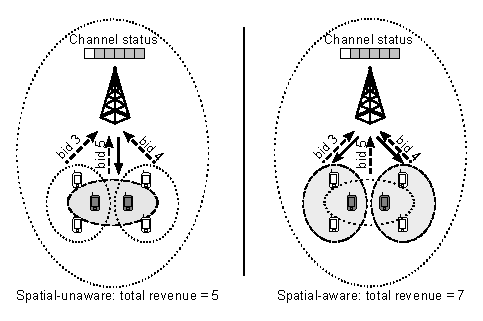
\includegraphics[scale=1.5]{Fig2.eps}
  \end{center}
  \caption{Example comparison of a spatial unaware and aware spectrum owner}
   \label{fig:SpecReuse}
\end{figure}

\subsection{Heterogeneity}
\label{subsec:Differentiation}
Spectrum heterogeneity \cite{ref:Gao2011,ref:Duan2011_Contract,ref:Xing2007,ref:Jia2008_com,ref:Niyato2008_Comp,ref:Min2011,ref:Dixit2010,ref:Niyato2007_Eq} refers to the consideration that different portions of the good have  different characteristics. This issue is explained in detail in \cite{ref:Xing2007}, but basically the idea behind it is that lower frequency signals travel better through obstacles and further at the cost of less amount of information transmitted and lower directivity for the transmission antennas. Another aspect considered to differentiate the spectrum is the continuity of the spectrum opportunity: it may consist of several, non-contiguous blocks, and the transmission hardware has a limit on the amount of discontinuous bands that can be used simultaneously. Finally, the spectrum QoS is perceived differently depending on the geographical distribution of the nodes or the amount of traffic carried in it.

All this leads to different valuations by users depending on their preferences and thus, it has an impact on their utility functions, demands and service selection (even selection of more than one operator \cite{ref:Jia2008_com}) which enable more niche markets that should be taken into account in pricing. For example, \cite{ref:Xing2007,ref:Min2011,ref:Dixit2010} include a physical propagation model (reflecting the heterogeneity of spectrum) into the utility functions of users, \textit{i.e,} utility depends on the received power at the SU receiver, and this power depends on parameters such as the central frequency of the channel assigned for that communication. Different channels sold by different spectrum owners would have different frequencies and thus, different valuations for the SUs.

Another example: \cite{ref:Niyato2008_Comp,ref:Niyato2007_Eq} include a parameter (``substitutability factor'') that represents the ability of users to switch frequencies freely within the spectrum. In a duopoly, the effect on the demands of the SUs would be as follows: 
\begin{equation}
D_i (c_i,c_j) = \frac{k_i - c_i - \delta(k_i - c_j)}{1 - \delta^2}
\end{equation}
where $D_i$ and $c_i$ represent the demand (for example, bandwidth) and cost per unit to the $i$-th operator, $k_i$ denotes the spectral efficiency or valuation of the SUs of the spectrum sold by the duopolists and $\delta$ is the substitutability factor. When $\delta$ is large, the demand to one operator is affected by the fluctuations in cost of the spectrum of the other operator, \textit{i.e.,} both spectrum chunks are interchangeable and users are free to switch from one to the other. In contrast, when $\delta$ is small, users are not as free and demands to each operator are independent. 

Another cause of heterogeneity comes from the side of users: most works consider users with different valuations of the good, mainly through the use of parameters in their utility functions such as the spectral efficiency or any other that indicates their different willingness to pay. Along this line, there are some works that take this idea further like \cite{ref:Xing2007}, which considers users more sensitive to quality or to price, or \cite{ref:Gao2011,ref:Duan2011_Contract} that classify users according to their channel conditions (causing different preferences about how much quality to buy), and \cite{ref:Yang2011,ref:Xing2007}, considering users with different and limited budgets.

\section{Formulation Frameworks: Proposed Solutions}
\label{sec:Math}

As we have shown, the designer of a spectrum trading mechanism has to decide: what objective should be optimized, which market mechanism should be used, and what special features of the spectrum as a traded good should be considered. 
In addition, the trading mechanisms can be mathematically characterized to obtain some insights into how each trading algorithm would achieve the design goals (although in the end, the ultimate objective is to improve spectrum utilization).  

When it comes to the mathematical model, there are several techniques available to formulate it.
The election of one or the other depends mainly on which of the issues of spectrum we are more interested in addressing and the preferred market mechanism for doing so.
Table \ref{Survey_table_market_formulation} shows what formulation frameworks are usually associated to each market mechanism, and the works applying these associations.
In this section, we explain which and how the characteristics of the spectrum trading scheme have been addressed by each modeling approach, highlighting the benefits and drawbacks of each one.

\begin{table}
\caption{Classification of papers by market mechanism and formulation framework}
\label{Survey_table_market_formulation}
\begin{tabular}{L{2.5cm}L{4cm}L{7cm}}
\hline
\textbf{Market mechanism} & \textbf{Formulation framework} & \textbf{Works} \\
\hline
Pricing & Game Theory & \cite{ref:Shen2013,ref:Zhu2012_Dyn,ref:Li2011,ref:Niyato2007_Game,ref:Niyato2008_Comp,ref:Niyato2009_Dyn,ref:Jia2008_com,ref:Ji2008,ref:Min2011,ref:Kaskebar2012,ref:Duan2011_Duo,ref:Duan2011_Inves,ref:Duan2010_Comp,ref:Duan2010_Cog,ref:Kim2011,ref:Dixit2010,ref:Tan2010,ref:Yu2010,ref:Maille2009,ref:Wang2008,ref:Xing2007} \\
				& Contract Theory & \cite{ref:Duan2011_Contract,ref:Gao2011,ref:Gao2013,ref:Duan2014} \\
				& Optimization & \cite{ref:Mutlu2008,ref:Yang2011}\\
				& Market-equilibrium & \cite{ref:Niyato2007_Hier,ref:Niyato2007_Eq,ref:Niyato2008_Mark,ref:Niyato2008_Spec,ref:Niyato2010,ref:Xu2011}\\\hline
Auction & Auction games & \cite{ref:Huang2006,ref:Zhou2008,ref:Huang2008_auc,ref:Wang2010_Spec,ref:Zhu2012,ref:Xu2010,ref:Sengupta2007,ref:Sengupta2009,ref:Illeri2005,ref:Jia2009_Rev,ref:Zhou2009_TRUST,ref:Wang2010_TODA,ref:Gao2011_MAP,ref:Wang2010_Spec}\\
\hline
Bargaining & Bargaining games & \cite{ref:Xu2012,ref:Yan2012,ref:Zhang2012_Fair,ref:Guijarro2011,ref:Pan2006}\\
\hline				
\end{tabular}
\end{table}

\subsection{Dominant Trend: Game Theory}
\label{sec:GameTheory}

Since the early works on spectrum trading, game theory \cite{ref:Myerson1997} has been the most used framework. 
\textit{Game theory} is a mathematical discipline studying situations involving individual rational decision makers (\textit{players}) pursuing their own (and often conflicting) objectives. 
In the framework of game theory, the interaction among these individuals is a \textit{game}. The actions (\textit{moves} or \textit{decisions}) made by the players bring outcomes (``payoffs'') to them.
The mapping of an action to every possible situation a player can perceive (\textit{information state}) is a player's \textit{strategy}, which can be, in general, random distributions over the action space. Agents are assumed to be rational in the sense that they will choose strategies that maximize, in expectation, their individual payoffs.

Clearly, the game theoretic framework matches the spectrum trading scenario.
For example, from the SUs' side, each user has the goal of maximizing its utility function by requesting a portion of a finite shared resource from an operator, at some cost. 
The fact of sharing a limited resource makes their actions to have an influence on each other. 
In this case, their interactions in spectrum trading can be seen as a game, where users are the players, their moves are their requests of spectrum opportunities and their payoffs are the value of their utility functions (\textit{e.g.} the data rate they get minus the payment to the PU).
This was indeed the origin of the works that used game theory in spectrum trading: it was used to study operators' resource allocation to secondary users in works that used pricing as the market mechanism.
For example, in \cite{ref:Niyato2007_Game}, the interaction between SUs when requesting spectrum to a primary operator comes from the price of spectrum, which depends on the total demand of all SUs. 
That is to say, the cost of a spectrum unit is determined by the amount of spectrum requested by other SUs, and this influences the amount of spectrum a particular SU requests. 
In \cite{ref:Yu2010} and \cite{ref:Wang2008} the spectrum opportunities are traded in the form of uplink power and the interaction between SUs is their mutual interference. 
On the other side, the cost per unit of spectrum was fixed by the spectrum owners using a different technique, optimization.

That research trend evolved to consider the spectrum owners'side also as a game, modeling their competition \cite{ref:Xing2007,ref:Maille2009,ref:Shen2013} and, as we remarked in section \ref{subsec:Market}, using other market mechanisms apart from pricing. 
Each spectrum owner has the goal of maximizing its profit function by exploiting its spectrum for its own use and/or selling part of it, obtaining some revenue for that. 
However, if there is more that one owner in an area willing to sell spectrum, they will compete for attracting buyers from a common pool of users. 
Then, for example under a pricing market mechanism, spectrum owners would be the players, their moves would be the price per unit of good and their payoffs would be the variation of their profit functions. 
Another parallel evolution was to use game theory in more complex markets, from the perspective of multiple secondary operators, to discover the best joint strategy for investing in spectrum from a primary operator and selling it to SUs \cite{ref:Jia2008_com,ref:Kim2011,ref:Zhu2012_Dyn}. 

\subsection{Most Frequent Game Theoretic Approaches}
The basic game theoretic formulation, considering a static one-shot game where agents have full information about other agents' actions and payoffs, is currently regarded as unfeasible to model most of the more complex situations in spectrum trading. Situations involving imperfect information, successive moves from the agents and the subsequent learning from past moves, and cooperation among agents.
In this subsection we focus on the approaches that are receiving more attention, and the cases where each one is applicable. These game theoretic models are:
\begin{itemize}
	\item Dynamic games.
	\item Auctions.
	\item Bargaining games.
	\item Contract theory.
	\item Cooperative games.
\end{itemize}

\subsubsection{Dynamic games}
\textit{Dynamic games} have been used from the beginning to deal with the issue of imperfect information. 
Dynamic games are a type of games where players interact more than once and they adjust their strategies based on what they have observed in previous rounds, \textit{e.g.}, from their own payoffs. 
The main advantage is that, in contrast to static games, players are not assumed to know information such as the actions taken by other agents and their payoffs. 
The drawbacks are that market is not cleared in one shot, and optimal solutions are not achieved under some circumstances, so their stability needs to be addressed. 

It is important to note that ``dynamic'' in most of these works means to go through several iterations in a fixed situation in order to converge to the solution of the equivalent static game with complete information. 
This is the case of the works using repeated games \cite{ref:Niyato2007_Game,ref:Niyato2008_Comp,ref:Niyato2009_Dyn,ref:Jia2008_com,ref:Ji2008}, where the same one-shot game is played several (or even infinite) rounds. 
Nevertheless, dynamic games offer more than this, such as the possibility of adapting the strategies to situations that change over time, such as variations in the supply and demand, or in the spectrum value (e.g. changes in channel gains) \cite{ref:Ji2006}.
Another aspect that can be modeled by a dynamic game (in the sense of time) is the transient period required by the players to achieve a stable equilibrium in works that focus on investing in spectrum and pricing strategies for secondary operators.
These works, that try to find the optimal joint strategies for investing in spectrum from a primary operator and selling it to SUs, consider multi-layered markets, as we will further explain in section \ref{subsec:Oligo}. These markets are studied as interrelated multi-stage games. 
An example could be a two-stage game where a lower stage models the operator selection of SUs and an upper stage models the competition of secondary operators in investing in spectrum from the primary operators. Until \cite{ref:Zhu2012_Dyn}, all works treated each stage independently, assuming the others had already reached equilibrium. 
And finally, players in a dynamic game could consider long term profits \cite{ref:Ji2008,ref:Zhu2012_Dyn,ref:Niyato2008_Comp,ref:Xu2012}.
This would bring results closer to optimality but at the cost of more complex formulations and computational overhead.

With an additional degree of difficulty, \textit{stochastic games}, a generalization of dynamic games which deal with uncertainty at a deeper level, are starting to be applied to spectrum trading \cite{ref:Shen2013}.
The main difficulties regarding stochastic games arise from the lack of a mature and complete theoretic framework, in contrast to other game theoretic techniques.
Not even approximate solution concepts, such as those based on multi-agent reinforcement learning, are assured to converge \cite{ref:Shoham2007}.

Even so, researchers are not focusing much on game theory applied to pricing now, as we said in section \ref{subsec:Market}.
This is in favor of other techniques that seem to naturally deal better with imperfect information such as auctions, bargaining and contracts, although these are subsets of game theory and also went through the previously commented evolutions.

\subsubsection{Auctions}
\textit{Auctions} can be described as games, played among the bidders, where imperfect information refers to the players true valuation of the item, and the strategies are the bids they are submitting to the auctioneer (see Section \ref{sec:TradedGood}). 
Although they have been applied to automated spectrum trading since the origins of its study, it is the technique that is receiving more attention nowadays. 
As we pointed out in section \ref{sec:TradedGood}, the main challenge of the works following this trend is to develop complex auction models under imperfect information, maintaining truthfulness and being computationally tractable in real time. 
An extensive survey on the topic can be found in \cite{ref:Zhang2012}.

\subsubsection{Bargaining}
With respect to bargaining, as we said in section \ref{subsec:Market}, it is only used in its one-on-one form in spectrum trading. 
\textit{Bargaining games} are a subset of game theory on their own but they can also be casted to an equivalent problem of another subset of game theory which is cooperative games (see section ``C.Operators bargaining - first phase'' of \cite{ref:Guijarro2011}. 
In bargaining games, the strategies of a player are the offers to make to the other entity and whether to accept them or not. 
Again, recently the idea is to incorporate dynamics to the bargaining model, so that it takes into account multiple negotiations with the same entity, trying to improve its solutions \cite{ref:Yan2011,ref:Yan2012}. Bargaining research is also in the direction of using it in multi-stage market models to speed up the trading \cite{ref:Guijarro2011,ref:Xu2012}. 

\subsubsection{Contract theory}
\textit{Contract theory} is a technique directly related to pricing.
In contract theory, the spectrum seller, rather than looking for an optimal price of spectrum, offers different spectrum items (for example, channels with different qualities) at different prices. 
If it offers the correct combinations of items and prices, the different type of users would respond according to their true valuations of the spectrum and the seller would optimize its revenue or social welfare.
The major drawback is that the spectrum seller still needs to have market power (be a monopolist).
This framework is currently making its first steps so the researchers' efforts are oriented to apply it to spectrum trading in diverse scenarios, specially in Cooperative Secondary Spectrum Access (CSSA, see section \ref{subsec:What}).

\subsubsection{Cooperative games}
Finally, it is worth saying that almost all works try to find sets of strategies that constitute an equilibrium of the game.
There are different types of equilibria (depending on the type of game), being the Nash equilibrium (NE) the most common. 
In an NE, no player has motivation to unilaterally change its current action because it would not improve its payoff. 
In other words, in an NE, the decision of each user is its best response to the decisions of the others (which are also best responses). 
But a particular NE does not necessarily entail optimality, that is, some or even all the agents would obtain a higher payoff with a set of actions that is not a NE.
Working in such an operation point (efficient outcome) would be desirable. 
To achieve this goal, it could be assumed that rational agents would be willing to reach an agreement to operate in an efficient outcome. 
When several or all the agents do that, we say that they cooperate, and the game is referred to as a \textit{cooperative game}.

Most spectrum trading works assume non-cooperative behavior, since it is natural to think that each user is on a free-for-all share of resources trying to maximize its satisfaction on its own, with no communication or help from other users, which are considered competitors.
However, sometimes this selfish behavior leads to inefficient outcomes (\textit{e.g.,} over-exploitation \cite{ref:Hardin1968}, or equilibria that are not optimal) and different techniques are used to drive players to better equilibrium points, mainly through some kind of communication between them. 
An example of these techniques are binding agreements ``enforced'' by a third party, such that it is in the best interests of all players to follow the recommendations of that party. 
The solution is called ``correlated equilibrium''. 
Despite it has been used in dynamic spectrum access \cite{ref:Han2007,ref:Maskery2009}, as far as we know it has not yet been exploited in spectrum trading works. 
Bargaining games are also an example of improving the efficiency of the outcome through communication.\footnote{``Bargaining games'' term is used here in a general sense and the improvement in efficiency they bring is compared to the efficiency of other games with the same number of players. That is to say, comparing multi-player games with no communication between entities to many-to-many bargaining games or comparing any other two player game with no communication to a one-on-one bargaining game. Multi-player markets as decomposition of multiple one-on-one bargaining games are less efficient than other multi-player games.} 
Another example are ``commitments'', where a player takes a binding action on him and informs the others so he can persuade them to take convenient actions to him. This would be the case of the leader in Stackelberg games. 

In a Stackelberg game \cite{ref:Simeone2008,ref:Zhang2009,ref:Yi2010,ref:Vazquez2010,ref:Duan2010_Cog,ref:Duan2011_Inves,ref:Zhu2012_Dyn,ref:Canzian2013} at least one of the agents, the ``leader'',  makes its decision first and the rest of the players (``followers'') react to it. 
The leader assumes rationality of the followers, so that they will choose their best possible responses after seeing the leader's decision.
Then the leader can force a situation where that best response of the players is one that is in the leader's interest. 
The solution to this game is the Stackelberg equilibrium, where the leader receives a better payoff than in a simultaneous game. 
The leaders of Stackelberg games may not only be the spectrum owners and the followers be the users, but also it can be used to model market where some entities have priorities over others, such as a partnership of a spectrum owner and a secondary operator \cite{ref:Zhu2012_Dyn}. 

Cooperative games, also called ``coalitional games'' (\cite{ref:Li2011} and a small snippet on \cite{ref:Xing2007}), go a step further in the relationship among players. 
Coalitional games focus on studying group utilities. 
They are closely related to dynamic games as shown in \cite{ref:Niyato2008_Comp}, specially infinite horizon games, where cooperation is encouraged due to the long term interaction that could be established among players and the possibility to punish in future actions those who do not respect agreements.
Coalitional game theory is also used to analyze collusive behaviors in \cite{ref:Ji2008,ref:Tan2010,ref:Sengupta2007}, when entities of the same type (spectrum owners on one side, or users on the other side) cooperate to affect market prices, harming the rest of the players and jeopardizing the efficiency of the system. 
Furthermore, \cite{ref:Tan2010} proposes a cooperation mechanism among small spectrum owners to fight against this price war. 
Unfortunately, we have not found many examples of cooperative games as we point out in Section \ref{sec:Open}.

\subsection{Alternative Frameworks}\label{sec:Deprecated}
In this subsection we discuss other approaches that have been considered an alternative to game theoretic formulation in the past but, for several reasons, do not currently receive the attention of the spectrum trading community. 
\subsubsection{Optimization}
\label{sec:Optimization}
Whereas \textit{optimization} has been widely used for dynamic spectrum access, only a few works in the past years have modeled a spectrum trading process entirely on optimization \cite{ref:Mutlu2008,ref:Yang2011}. Optimization, also called ``mathematical programming'', is the search of the best values of some parameters such that selected objective functions are maximized or minimized, subject to a number of constraints. 
The main difference between game theory and these works is that the latter does not consider the other agents as rational decision makers, \textit{i.e.} as independent agents pursuing their own objectives. 

Note that this idea does not imply a tyrannical attitude from the spectrum owners. 
In fact, it is still interesting for them to make the trading incentive-compatible for these users, either because nobody would buy its services otherwise or because a regulator may enforce this type of optimization.

In the context of spectrum trading it is developed in a single spectrum owner market form (monopoly).\footnote {It could also be carried out by a third party, a regulator authority, although no examples have been found of that, probably because that would not be accepted by the entities involved as they would not have any way to influence it.}
The parameters to look for are usually price per commodity unit (often bandwidth or power), the constraints to respect are related to degradation caps on PUs' activity and the goal of the optimization could be as diverse as pointed out when describing the design of trading mechanisms (see section \ref{subsec:Market}).

The main advantage of optimization is that, in theory, it could achieve the best solution among all techniques described, from a system perspective or in the case of only one decision maker with market power (a monopolist). The definition of ``best'' depends on the objective of the optimization, and thus, of that trading mechanism (see section \ref{subsec:Objective}): \textit{e.g.} best in terms of the sum of the utility functions of all users, or in terms of fairness, best from the PU monopolist perspective in terms of its revenue, etc. 
Nevertheless, that is only possible in very simple models. 
It suffers from the ``curse of dimensionality'' and models become easily intractable, as explained in \cite{ref:Ji2006}.

It is interesting to note that optimization is usually combined with other frameworks: it has been used for setting prices in monopoly works that used game theory for resource allocation among SUs (see section \ref{sec:Market}) and it is necessary for computing equilibria in games, for determining the winner of an auction, etc. 

The efforts are mostly oriented to formulate the problem as a convex optimization problem (the objective function and the constraint sets are convex).
Convexity has notable mathematical advantages and make very large optimization problems tractable.
If the problem is non-convex, in general, simpler versions of the problem (sub-optimization) are solved.

When the decisions are made over stages, or time-slots, the optimization problem can be solved by means of a decomposition principle known as \textit{dynamic programming}. 
This is the single-agent equivalent to a dynamic game. 
In spectrum trading this framework has been used in \cite{ref:Mutlu2008} to model a spectrum trading system as a Markov Decision Process (MDP). 
An MDP models uncertainty introducing system states and rewards that are not completely determined by the actions taken in each stage (partially random changes).  
A stochastic game is a generalization of an MDP to multiple decision makers. 
Compared to non-dynamic frameworks, the optimal strategy solving an MDP is farsighted, and therefore better in the long term than a strategy that only optimizes the payoff obtained in the current stage (myopic strategy).

\subsubsection{Market-equilibrium}
\label{subsec:marketeq}
Borrowed from microeconomic theory, D. Niyato and E. Hossain develop in \cite{ref:Niyato2007_Hier,ref:Niyato2007_Eq,ref:Niyato2008_Mark,ref:Niyato2008_Spec,ref:Niyato2010,ref:Xu2011} a solution to the conflict of interests between a single buyer and a single seller, later extended to the multiple buyers and sellers case.
It is based on the demand and supply theory: differentiating the profit function of the seller with respect to the amount of good to trade, a supply function $S(c)$ can be obtained which expresses how much of the trading good should be sold given a price in order to maximize its satisfaction. 
Similarly, a demand function $D(c)$ can be obtained for the buyer, differentiating its utility functions with respect to the amount of good to buy, showing how much of the trading good should be bought given a price in order to maximize its satisfaction. 
The intersection of both functions is the \textit{market-equilibrium}, where supply equals demand.

Solving that equation may imply having perfect information of the network (\textit{e.g,} the demand function could depend on the channels gains) which is a hard constraint to meet in a real environment, so they proposed several distributed and iterative learning algorithms to reach that solution. 

In \cite{ref:Niyato2008_Mark}, the authors compare the market equilibrium mechanism against two other approaches, competition and cooperation among entities.
Their results show that market-equilibrium is the most stable approach and implies a low communication overhead, at the cost of a lower profit for the spectrum sellers and lower social welfare, as well as certain requirements on the available bandwidth for sale (otherwise equilibrium will not exist).

In \cite{ref:Niyato2007_Hier} the authors extend the idea to create interrelated multi-level markets where there is a first market between primary and secondary services, another between secondary and tertiary (because the secondary can also sell spectrum opportunities) and so on. These multi-level markets may be different categories of services or multi-hop networks. A practical point of view is presented in \cite{ref:Niyato2010}, where the authors apply their model to an integrated WiFi-WiMAX network as in Fig. \ref{fig:WiFi-WiMAX}. In this practical example, a WiMAX base station (primary provider) offers delay-sensitive access as its primary service, but it can also sell secondary access in the form of loss-sensitive connections. The bandwidth available to sell to secondary providers depends on the PUs' demand and that trade-off is expressed in the primary provider profit function. The secondary providers are able to re-sell that spectrum to a tertiary service provider at the same time, in a similar trade-off to the one that faces the primary service. This tertiary service provider is a best-effort WiFi access point. This work is specially interesting because it shows the application of their trading algorithm to a specific scenario and technologies. 

This technique has not been completely abandoned since the work in \cite{ref:Xu2011} is from 2011 and extends the idea further by applying this market equilibrium model to a market with several entities that can buy and sell spectrum and other features as spatial reuse, budget constraints and multiple channels to buy/sell.

\begin{figure}[ht]
	\begin{center}
  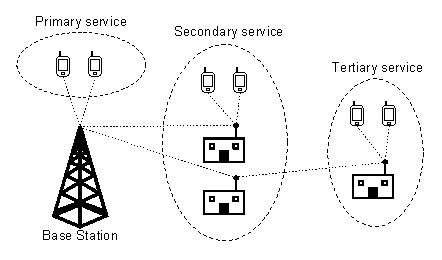
\includegraphics[scale=1]{Fig3.eps}
  \end{center}
  \caption{Application of \cite{ref:Niyato2010} to a WiFi-WiMax network}
   \label{fig:WiFi-WiMAX}
\end{figure}

We present in Fig. \ref{fig:frameworks} a diagram summarizing the trade-off between how satisfactory the solution of a particular scenario is with each framework and how difficult it is to implement in a real scenario due to the communication and computation overheads (with regard to trades in real-time). 
This figure also features the research status of each approach. 
The color of each circle is related to the attention that the technique is currently receiving and the size of the circle is proportional to the amount of works using this technique.
Our conclusion, as we develop in the final section of the chapter, is that attention should now be directed more to the practical issues of implementing spectrum trading algorithms rather than trying to push their analytical optimality forward: the key of automated spectrum trading should be adaptability to time-varying spectrum and self-organization (distributed, local based algorithms), not only to ``make them happen'' with the real phenomena they have to deal, but also to convince actual and potential spectrum owners, who are the ones that would have to actively adopt them in the end. 

\begin{figure}[!ht]
  \begin{center}
  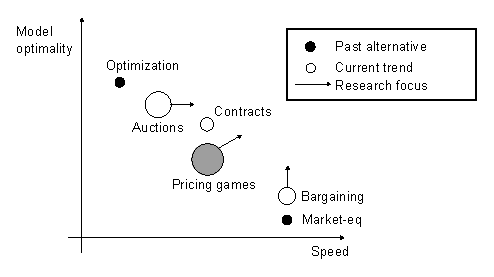
\includegraphics[scale=1.25]{Fig4.eps}
  \end{center}
  \caption{Formulation frameworks: optimality of solutions versus implementability. The size of each circle represents the amount of works in the area. Game theory (pricing) is shaded because interest in it is decreasing}
   \label{fig:frameworks}
\end{figure}

\section{Market Forms: Possible Situations of the Market.}\label{sec:Market}

In this section we present some spectrum trading systems with an holistic view, focusing on the entities involved and the relationships they establish between each other. We classify them in \textit{monopoly} and \textit{oligopoly} markets, based on the number of spectrum sellers (see table \ref{Survey_table_market_form}).

\subsection{Monopoly}
\label{subsec:Mono}
In a monopoly situation only one entity operates as spectrum seller without any competition, and multiple SUs buy the spectrum opportunities offered by this single entity.

This situation is clearly less favorable for the spectrum buyers than the case of multiple sellers, where an increased competition would lower the prices and spectrum would be used in a more efficient way. However, it can be found in many practical situations, \textit{e.g.,} if only one operator is willing to trade its spectrum; if there are several spectrum sellers and all but one are congested with primary traffic; if in a given area only one operator has infrastructure to provide coverage in the spectrum bands that are traded.

The most common market mechanism in this situation is pricing, where SUs make their own decisions about the amount of spectrum they want, although their actions may influence each other. In this case, SUs are modeled as agents in a game-theoretic formulation. On the other hand the monopolist optimizes the spectrum price, assuming it knows how SUs would react to the price. Most works consider the actions of the monopolist as part of the game \cite{ref:Simeone2008,ref:Jayaweera2009,ref:Zhang2009,ref:Jayaweera2010,ref:Vazquez2010,ref:Yi2010}.

We have previously mentioned that the game theory pricing approach evolved to contract theory in order to handle the imperfect information issue. L. Gao \textit{et al.} in \cite{ref:Gao2011} and later together with L. Duan \textit{et al.} in \cite{ref:Duan2011_Contract} introduced and developed the concept of ``quality discrimination spectrum trading'': a spectrum trading market where SUs are classified into multiple (discrete) categories according to their preference for a given spectrum quality when buying a channel. In the specific case considered in these works, ``quality'' stands for the maximum allowable transmission power. All computational effort lays at the monopolist's base station or access point, which has to obtain the optimal set of qualities-prices and associate them to each SU consumer type, so that PU's revenue is maximized while making these associations (called ``contracts'') compatible with the interests of the SUs, \textit{i.e.,} each SU from a type should consider its assigned quality-price as its best option, even considering not to transfer at all.

Another popular approach in monopolies are auctions, \cite{ref:Huang2006,ref:Zhou2008,ref:Huang2008_auc,ref:Wang2010_Spec,ref:Gopinathan2011,ref:Zhu2012,ref:Jia2009_Rev} where the winner determination is formulated as an optimization problem for the monopolist. For the SUs, two approaches can be identified: in truthful mechanisms, they only have to submit their true valuations of the traded good \cite{ref:Zhou2008,ref:Gopinathan2011,ref:Zhu2012,ref:Jia2009_Rev}; in other works, the bids submitted by the SUs correspond to the outcome of a game played among them \cite{ref:Huang2006,ref:Huang2008_auc}.

Other models rely entirely on optimization, such as \cite{ref:Mutlu2008}. In that work the monopolist uses dynamic programming to obtain policies on when to allow or block SUs access to its channels, considering that the price charged will vary as a function of the occupation of the system. That variation on the charged price will also influence the arrival rate of SUs (decreasing with price).

A fully decentralized approach is presented in \cite{ref:Wang2008}, where SUs are modeled in a non-cooperative game to determine the amount of power they are using to transmit (power is the traded good), given a price, which is computed by each user in a distributed fashion, using only local information (e.g, channel gains of its neighbors), avoiding the need of global information. The monopoly part of \cite{ref:Yang2011} proposes a distributed optimization similar to \cite{ref:Wang2008} among the monopolist and the SUs, where the monopolist computes part of the parameters for the pricing and broadcasts them to the SUs, which infer the rest. 

\begin{table}
\caption{Classification of papers by market form.}
\label{Survey_table_market_form}
\begin{tabular}{L{3cm}L{11cm}} 
\hline
\textbf{Market forms} & \textbf{Works} \\
\hline
Monopoly& \cite{ref:Niyato2007_Game,ref:Mutlu2008,ref:Wang2008,ref:Yu2010,ref:Gao2011,ref:Yang2011,ref:Xu2012,ref:Huang2006,ref:Zhou2008,ref:Huang2008_auc,ref:Wang2010_Spec,ref:Gopinathan2011,ref:Zhu2012,ref:Simeone2008,ref:Jayaweera2009,ref:Zhang2009,ref:Jayaweera2010,ref:Vazquez2010,ref:Yi2010,ref:Duan2011_Contract,ref:Duan2010_Cog,ref:Duan2011_Inves,ref:Jia2009_Rev} \\\hline
Oligopoly & \cite{ref:Li2011,ref:Xu2012,ref:Xing2007,ref:Jia2008_com,ref:Niyato2008_Comp,ref:Maille2009,ref:Duan2010_Comp,ref:Duan2011_Duo,ref:Zhu2012_Dyn,ref:Guijarro2011,ref:Min2011,ref:Kim2011,ref:Tan2010,ref:Dixit2010,ref:Xu2010,ref:Sengupta2007,ref:Sengupta2009,ref:Illeri2005,ref:Wang2010_TODA,ref:Gao2011_MAP} \\
\hline
\end{tabular}
\end{table}

\subsection{Oligopoly}
\label{subsec:Oligo}
A monopoly may not be the most usual situation, as it is highly likely that, in a region, more than one spectrum owner will be interested in selling, and furthermore, it is a desirable situation from the point of view of resource exploitation and users' welfare because, in general, sellers competition lowers prices. 

However, setting up a competitive spectrum trading market is not easy. As licensed spectrum owners' profit diminishes, they would be willing to use aggressive market strategies to eliminate competition and end up as monopolists or to forbid entrance to newcomers. For example, licensed operators may acquire spectrum not to increase service quality or to provide a new service but to make the others fail to acquire it and thus lose their competitive power. Or, they may acquire extra spectrum to speculate with it: obtaining benefit from the trading itself. Collusions, as we introduced in section \ref{sec:Math} when describing cooperative games, also belong to this category. 

To avoid these issues, a well designed and enforced regulation can help to encourage and protect competition while keeping incentives for spectrum owners. This issue is addressed in \cite{ref:Yoon2012,ref:Tan2010}. In particular, in \cite{ref:Yoon2012}, this effect of competition can be seen in a comparative study of secondary-use frameworks (auction, pricing and brokerage). The authors also propose and analyze the effect of a maximum amount of spectrum trading on the different frameworks and show when each of them is more convenient to use depending on the state of maturity of the market. They argue that the final objective should be to use pricing, as it is the one that produced better results under their experiments, considering not only profits but fair competition issues, users' utilities, and spectrum efficiency. Aggressive strategies are studied in  \cite{ref:Tan2010} from two perspectives: the short-term aggressive strategies to capture more users of the market and the long-term predatory pricing. It also shows a cooperative responding strategy for the smaller spectrum owners to avoid monopoly. 

\subsubsection{Three-layered market model}
Competition among sellers is introduced in most of these works on a three-layered market model as in Fig. \ref{fig:LayeredMarket}, composed of spectrum owners whose spectrum is licensed by a regulatory entity (such as the FCC) and provides service to a set of PUs on long term subscriptions, and secondary spectrum operators which buy unused spectrum to the primary providers and sell it to SUs in a typically shorter time basis (even real-time/on demand). The first layer of the market is the (generally auction) process where primary operators (POs) get spectrum licenses. 
In the second layer those operators sell portions of their spectrum to the secondary operators (SOs).
In the third layer market, which operates with the smallest time-scale, the SOs sell their services to the end users over the leased spectrum. 

The market layers should not be confused with the number of game stages modeling these markets. Considering that the focus is in the second and third market layers, the game usually comprises three stages: spectrum investment (SOs buying spectrum), spectrum pricing (SOs setting a price) and demand distribution (SUs selecting SO). However, a market model can have more than three layers, by allowing SUs to re-sell spectrum, establishing ternary, quaternary markets, and so forth. Most works on this section focus on SOs.

\begin{figure}[!ht]
  \begin{center}
  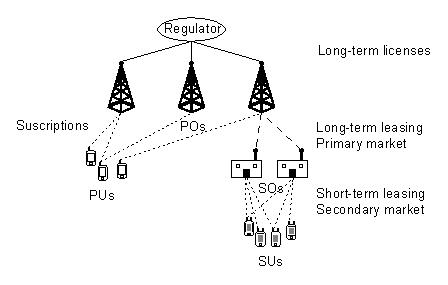
\includegraphics[scale=1.25]{Fig5.eps}
  \end{center}
  \caption{Three-layered market}
   \label{fig:LayeredMarket}
\end{figure}

The reason of existence of these virtual\footnote{``Virtual'' as they have no spectrum license and may not even have infrastructure as a Mobile Virtual Network Operator ``MVNO'' for cellular networks.} intermediaries to do the secondary trading is that they could focus on it, being near the end costumer and thus, crafting tailored plans and/or adding innovative or exclusive services \cite{ref:Duan2010_Comp,ref:Levi2012}.

In addition, intermediaries provide a way to ease the entrance to the market to a new PO and therfore, to improve users' welfare and spectrum utilization as well as providing incentives for existing POs since it gives them the option of selling their bandwidth excess without having to worry about designing pricing and/or marketing plans for SUs to buy it. 

Some works introduce competition into the pricing problem and focus on this middle layer by jointly studying spectrum investment and pricing \cite{ref:Jia2008_com,ref:Duan2010_Cog,ref:Duan2010_Comp,ref:Duan2011_Duo,ref:Duan2011_Inves,ref:Kim2011}\footnote{Works \cite{ref:Duan2010_Cog,ref:Duan2011_Inves} do not really study sellers' competition but they are closely related to other works featured in this section, showing the same structure and dealing with investment as if they were on a competitive environment.}. There are also works outside this three-layered market model \cite{ref:Illeri2005,ref:Xing2007,ref:Maille2009,ref:Dixit2010} even with a different relation between primary and secondary operators \cite{ref:Guijarro2011}.

Focusing on SOs as intermediary entities, it is interesting to evaluate the impact of the price they pay to the spectrum owners on the final price charged to SUs. There are several issues of concern around spectrum investment: some works like \cite{ref:Jia2008_com} assume that, no matter if the spectrum is bought to the regulator or to PUs, these are long-term transactions (\textit{i.e.,} for years), a legacy from the old command-and-control law framework, while SOs are looking to satisfy SUs' needs almost on demand. Therefore SOs try to adapt real time dynamic pricing strategies for SUs to those long-term investment decisions. Another point of interest is that competition can also take place at the investment stage among SOs either directly, where they are trying to get ``best quality'' spectrum, \textit{e.g,} \cite{ref:Kim2011}, and/or they are charged based on their aggregate demand \cite{ref:Jia2008_com}; or indirectly, as the bandwidth amount offered by each operator to the SUs and its aggregate total will influence prices and profits \cite{ref:Duan2010_Comp}. And while most of the works on spectrum trading only consider leasing as the way to obtain spectrum, L. Duan, J. Huang et. al. have studied the influence of spectrum sensing in \cite{ref:Duan2010_Cog,ref:Duan2011_Inves} as an additional way to obtain spectrum, proving that this possibility always increases SO's expected profit and users' payoffs. 

Another alternative is sharing a spectrum band, proposed in \cite{ref:Maille2009}, where two operators have a fixed (licensed) part of spectrum and an unlicensed common band which can be used under congestion and for free. Their results show that when the unlicensed to licensed band ratio increases, the profit of the providers decreases as well as the social welfare. On the other hand, users' welfare increases, so it is the role of the regulator to fix the amount of shared band in this trade-off.

\subsubsection{Other market models}
Several works show a different market structure. In \cite{ref:Illeri2005} a variation of a private commons regime is modeled (the authors call it ``mixed commons/property-rights'') with a centralized Spectrum Policy Server (SPS) per geographic domain. When each user enters the system, it connects to this broker which obtains its location and a function called ``acceptance probability of services'' related to its utility function. Then, the SPS starts an iterative bidding process of service offers from operators where the winning bid is the one with the highest acceptance probability, which is shown to the user and accepted with that probability. An extension to a multi-user environment is also studied. The authors of \cite{ref:Xing2007} consider that a centralized controller does not match the reality in a system that is distributed by nature and proposed a similar model with operators and users interacting directly. In \cite{ref:Dixit2010}, the authors are also interested in a different market model, without brokers or any centralized entity, where the primary base stations should be the ones to also serve SUs by selling them primaries' unused spectrum directly. The authors of \cite{ref:Guijarro2011} are close to the three-layered market model (it is a three-layered market indeed) and study DSA but in a \textit{Mobile Virtual Network Operator} fashion, \textit{i.e.,} when the virtual operator buys spectrum to the licensed one, it becomes its competitor for a common pool of users and both play a non-cooperative game on the price per subscription charged to those users.


\section{Open Research Lines and Future Trends}
\label{sec:Open}
Based on the drawbacks of current proposals, which we have pointed out in the preceding sections, and considering the issues that are recently receiving more attention from the research community, we would like to highlight the following unresolved challenges: 
\subsection{Real-Time Adaptation Versus Optimality}
In spectrum trading research, the main tendency has been building increasingly complex models, which deal with more issues of spectrum in more convoluted markets, and aiming to solve them optimally.
Nonetheless, the resources required to reach such elaborated solutions have not been considered enough, specially time. 
Time consumption is a relevant issue because, as we have been pointing out throughout our survey, multiple important parameters in spectrum trading experience rapid variations over time: spectrum opportunities, demand (unplanned peaks of traffic), valuation of the spectrum (changes in channel gains, mobility of entities), etc. 

In consequence, we think that time consumption should be regarded as a key feature in spectrum trading algorithms: if obtaining an optimal solution takes so long that the system's parameters vary significantly during the computation time, this solution will be not optimal when applied.
In addition, the more time devoted to negotiation among the agents, the less time used in transmission. 
For that reason, it is more practical to design models that may not fully exploit spectrum in a particular moment (for example, by not taking into account spectrum geographical reuse) but that are capable of reducing the uncertainty due to the changes over time, and thus, providing higher guarantees on the agents' satisfaction. 

According to the computation and communication overhead, it would be fair to say that the most suitable frameworks to achieve real-time adaptation are those that are decentralized and compute solutions based on local observations (imperfect information), otherwise it would imply lots of entities communicating with a central node. 
Despite that idea, achieving real time operation in complex auction models is a hot topic in spectrum trading research \cite{ref:Vidal2013,ref:Kim2013,ref:Xu2012}. 
This is due to the fact that optimality is still in the spotlight, as pointed out in \cite{ref:Vidal2013}: ``The decentralized approach has several advantages that make it attractive: lower complexity than the centralized approach, robustness and scalability. 
However, with decentralized approaches there is no guarantee that optimal solutions can be achieved. 
To optimize objectives, such as global efficiency and fairness, and some important parameters, such as price of anarchy and price of stability, the spectrum data for all SUs in the network should be considered''

Nevertheless, two approaches are, in our opinion, more promising to overcome the time-efficiency issue: bargaining and contract theory. 
One-on-one bargaining offers simplicity on its algorithms, while it can be extended to include more features such as dynamic behavior and adaptation: the bargain process can be made over several stages in order to reach better agreements, and it can take into account past trading history and far-sighted decision making \cite{ref:Yan2011}. 
When multiple agents interact, one-on-one bargaining is not optimal in general (many-to-many bargaining is indeed optimal, but is a much more complex problem, lacking the simplicity and efficiency of the one-to-one scheme), as it is not considering all available entities and relationships as a whole. 
But the negotiation among pairs can be easily done in real-time, so that there are no utility losses because of computational or communication delays. 
In order to compensate the sub-optimality of this approach, it is possible to study beforehand which pairs of entities are best matches to each other (rather than matching pairs randomly).
  
Many-to-many bargaining is studied as a cooperative game where all entities must be committed to the agreement, and therefore deviating from the \textit{grand coalition} should not be in the interest of any subset of entities. 
It appears to be less tractable because it would require intense message exchange between the members of the coalition.
Cooperative games in general, however, are interesting because they can look for higher and longer term utilities (allowing Pareto optimal outcomes). 
	
Pricing was seen as an effective way to deal with time variations, as each entity could compute the optimal price on its own and then users would choose the most convenient for them. 
However, it its simplest form, its algorithms required much knowledge about the network: for example, price was established based on how much users value spectrum (their demand) and that information is unlikely to be shared. 
Users could play strategically with that in order to get lower prices by reporting lower valuations. The price menu offered by contract theory tackles that imperfect information and maintains decentralization and low communication, although, again, it comes at the cost of lower utilities with respect to an ideal global optimization. 

\subsection{Implementation and Applications}
Almost all the efforts on spectrum trading research have been devoted to the analytical study of the economic aspects of the trading. 
It is true that other related technical challenges, such as spectrum sensing or MAC protocols \cite{ref:BWang2011,ref:Domenico2012}, to cite some, are studied in cognitive radio papers, but are hardly found in spectrum trading works. 
However, combining technical and economic aspects in trading mechanism research, even in prototype design, would throw light on relevant, non-trivial issues.
For example, how to put together the stages of a MAC protocol with those of the spectrum trading algorithms, that is to say, how the trading algorithm translates into an exchange of control packets. 
In fact, these issues may have an impact on the performance of the trading algorithm such that it needs to be tuned (\textit{e.g.} to handle or reduce time delays). 
Nevertheless, these implementation issues have received little attention (unlike, for example, the authors of \cite{ref:Wang2008}, who designed and described a practical MAC protocol for their algorithm). 
In contrast, there have been numerous MAC proposals \cite{ref:Domenico2012} for dynamic spectrum access with cognitive radio. 

The same happens with regard to applications of these models in practical network environments with specific wireless technologies. 
There are only few works that consider that in spectrum trading (IEEE 802.22 standard-based wireless regional area networks in TV white spaces in \cite{ref:Niyato2010}, Wi -Fi and WiMax in \cite{ref:802}).
Because of the issues and challenges discussed in previous sections, it would be fair to say that implementation and applications of spectrum trading would need more than a simple extension of the models for dynamic spectrum access without trading.

And all this is particularly important because it threatens the main reason of existence of spectrum trading: creating an incentive to incumbent operators.

\subsection{Incentives to Incumbent Operators}
As we stated in the introduction, there are some other ways to optimize the use of spectrum apart from automated spectrum trading, such as a forced dyamic spectrum access. What makes spectrum trading different from other proposals is that it creates incentives to spectrum owners so that they would be willing to facilitate the access to their unused spectrum to other secondary entities. 
Creating incentives instead of forcing the operators avoids that actual spectrum owners as well as prospective ones feel discouraged from investing in new spectrum technologies and services: ``why am I going to spend money in spectrum if the government is going to give it for free to others?''

Therefore, it is needed that these operators believe in an automated mechanism that controls their profits. 
But this idea alone is scary. ``Is there any security on obtaining benefit''? The short answer is ``yes'' but the long answer would be ``only in theory''. 
It is hard to convince he telecommunications industry to adopt spectrum trading if there are no test-bed experiments and there is no strong evidence that these algorithms do not lead to economic loses (due to dis-adaptation to real time, for example). Optimality, then, remains in the background. 

On the other hand, secondary users also need an incentive to request spectrum from the primary operator (\textit{e.g.} inexpensive tariffs). Otherwise, the trading market will not work because they would all prefer to become primary users. 

In a different and complementary approach, something can be added to money as an incentive to spectrum owners: services, specifically, secondary users acting as relays in Cooperative Secondary Spectrum Access (as we have pointed out in section \ref{subsec:What}). 
Albeit money is always an incentive and satisfaction due to it never saturates, this adds a new and non-substitutable reason for sharing: \textit{e.g.} secondary users can act as relays for increasing the primary operator range. 
Furthermore, the most promising feature of CSSA is using it when the primary operator is congested, in order to increase its transmission rate. 
Due to that increase, new spectrum opportunities would be generated and there would be more spectrum sharing and efficiency. 

However, CSSA provides no incentive to primary operators when they have low traffic volume and they are not interested in augmenting their transmission rate.
For that reason, hybrid approaches of CSSA and economic exchanges are being studied \cite{ref:Zhang2012_Fair,ref:Zhang2009}. 
New approaches are also exploring the idea of offering other services to the primaries like secure transmissions \cite{ref:Lee2011} or offload services \cite{ref:Pantisano,ref:Yi}

\subsection{Protection Against Malfunctions}
Along the same line of implementation issues, it is not difficult to think that a system is likely to behave differently as planned due to intentional or unfortunate events.
\subsubsection{Intentional failures: untruthfulness and collusions}
Although, like every aspect of social interactions, spectrum trading would have a regulation framework protected by the law, it is by no means irrelevant to design mechanisms that prevent or discourage market manipulation. It is so because of the precautionary principle (i.e. ``better to be safe than sorry''), it is easier to be proactive and avoid such situations; and most of the times market manipulation could be hard to prove: for example, if an algorithm depends on entities reporting their true valuation of the spectrum, how could someone prove that they are being untruthful?

As we have previously commented, truthfulness has been studied for a few years and it is still a hot topic. The essential problem here is that combining truthfulness with some other goals such as real time, optimality, spatial reuse, etc. soon makes the algorithm intractable and there is no accepted solution to that so far.

Collusions, cooperation of a set of players to influence market prices and harm the others, have received little attention, perhaps because they could be more easily spotted by a regulator authority, as it has happened in other markets. 
They are, however, a serious threat to the correct operation of the system, not only because it may turn it inefficient, but also because it can end up ruining the non-colluding entities, erasing competition and destroying the market.

\subsubsection{Unfortunate events: lack of rationality}
Failures can also occur in a system when control information is not correctly received due to propagation issues or contains any error from the source. 
This event would not only cause immediate loses or suboptimal trades but it can also push the system to a permanent situation of inefficient operation. 
All approaches assume that entities are rational and do not study the impact of such failures. They also do not consider the implementation of reactive mechanisms to make decisions under the irrational behavior that would take place. 
To the best of our knowledge, there are no published works addressing this aspect of spectrum trading.  

Furthermore, even without considering erroneous information, irrational behavior may take place. 
In section \ref{sec:Optimization} we explained how optimization was discarded as a main tool to model spectrum trading because it was affected by an inherent ``curse of dimensionality'' .
Then, game theory, showing a decentralized approach studying entities as individual rational decision makers, became the preferred method. 
Sadly, the applicability of game theory beyond very limited models and the whole concept of finding an equilibrium are being called into question. 
In fact, \cite{ref:Galla2013} suggests that failure to converge to equilibrium in some complex games is independent of the learning algorithm and the behavior of players ends up being essentially random.

\subsection{Complex Game Models}

This point could be considered as a contradiction with the previous one, where we cited how complex game theory models may not be tractable.
Nevertheless, we still think that some complex formulations have not been explored enough yet and feature some promising properties so as to conclude they should not be abandoned this soon. 

We showed that a method to deal with the uncertainties of spectrum is trying to reduce it with simple (not necessarily optimal) real-time algorithms. 
However, it is not the only way to do so. 
Another way to do it is thinking about long term rewards and relationships using cooperative games. 
Cooperation and considering the history of play gives the feel that it is a more secure and profitable system: cooperation allows to reach higher profits than competition, allows fair sharing of revenues, there are punishment strategies if someone deviate from coalitions, etc. 
But the drawback has already been stated: ``coalitional games are inherently difficult to solve'' \cite{ref:Li2011}.  In addition, they require more communication between the entities which may push them far away from real time and may creat a dis-adaptation that may not be compensated with the long term commitments. 

A promising way to achieve the benefits of cooperative games but with smaller computation and communication overheads, could be to maintain some local measure of ``reputation'' about the other players as in \cite{ref:Yan2011}.
Reputation is a way to ``compress'' past histories, expressing how likely is to achieve a good transaction with those other players and thus, it can be used to prioritize one player over the others. 
That would encourage every involved entity to share its resources. 

Another interesting research line is exploring the effect of transient times in multi-stage games. 
An example of a multi-stage game could be that of an oligopoly of spectrum providers serving to a common group of users: at one stage, the users perform the service selection according to the prices and perceived quality; at the next stage, service providers decide the spectrum to lease and its price. 
Both stages are interrelated but almost all works solve them by backward induction, assuming that one of the stages is in equilibrium before including it in the other stage game. 
In reality, both dynamic stages would be looking for equilibrium at the same time and considering the impact of such transient states could increase profits and reduce the convergence time, at the cost of a more complex formulation \cite{ref:Zhu2012_Dyn}.

Lastly, stochastic games deal with uncertainty by trying to incorporate it to the model. 
However, as we pointed out before in the survey, they are still a subject of research for theoretical mathematicians so its use in spectrum trading requires more than trying to apply it and still lacks of a more complete theoretical foundation. 

\subsection{Complex Market Joint Studies}
We have shown in section \ref{subsec:Oligo} that the most common market model in spectrum trading works is the three-layered one of Fig.\ref{fig:LayeredMarket}; where the spotlight is put on the decisions of the secondary operators in the middle layer. 
Even if this structure is not followed, a very extended assumption is that a primary operator provides service to its subscribers (primary users) and sells unused spectrum to a secondary operator who, in turn, tries to convince other entities (secondary users) to pay for the services provided over its leased spectrum. 

But in reality, users are not primary or secondary by default: an entity willing to use spectrum would consider to become a primary user paying a subscription to a primary operator or become a secondary use served by a secondary operator. 
Each service profile is different: the one of the primary operator is more reliable, possibly with a higher transmission rate and better QoS. 
On the contrary, the secondary operator could possibly be more aggressive in price. 
The point is that there are some unexplored interactions such as a primary owner considering that when it its selling spectrum to a secondary operator, it becomes its competitor as in \cite{ref:Guijarro2011}, or a primary operator dealing at the same time with primary and secondary users \cite{ref:Dixit2010}. 
And on the users side, for example, the idea of users selecting which network they prefer, primary or secondary \cite{ref:Elias2013}.

These overlooked considerations are indeed relevant in a real scenario and could be used to boost the efficiency of a trading market, or, at least, keep it working: let's imagine a secondary operator offering the most suitable service to users such that these users would never decide to turn into primary users, starving the primary operator. 



%\item Implementation and application of the models: most of the effort on spectrum trading research has gone to the economic aspects of the trading. Nevertheless, technical issues such as developing MAC protocols \cite{ref:Wang2008} have received little attention. In contrast, there have been numerous MAC proposals \cite{ref:Domenico2012} for DSA with cognitive radio. The same happens with regard to applications of these models in practical network environments, there are only few works that consider it for spectrum trading \cite{ref:Niyato2010,ref:802}. Because of the issues exposed in the works we show, it would be fair to say that implementation and applications of spectrum trading would need more than a simple extension of the models for DSA without trading.
%\item Communication overhead: along that line, the associated cost to information exchange among agents in order to perform the trading is not usually considered \cite{ref:Xu2010,ref:Niyato2008_Mark}, understanding ``cost'' as delays that prevent real time trading and other resources needed to do so (such as power).
%\item Protection against misconducts or nasty agents: most of the spectrum trading algorithms are still based on the knowledge of the agents' private information and/or trusting that they would report their true valuations. As it has been previously pointed out, in reality they have incentives to transmit misleading information so that they would increase profit at a cost of unfairness, system disequilibrium, etc. Combining this objective with efficient allocation of resources remains as an open problem. Other negative situations could be malicious collusions among providers or users to rise/lower prices.
%\item Modeling of complex interactions: most works on spectrum trading consider a one-shot interaction among agents where policies are computed offline. They do not take into account ideas such as future payoffs, priorities on trading due to previous agreements, online learning of policies, communication among agents (cooperation), etc. Taking into account previous trading history as well as forecasts about the future or any other complex relationship could maximize long-term satisfaction. There are mathematical tools to implement this but it has received little attention, perhaps due to the additional complexity they introduce which may make problems computationally intractable (as with truthfulness and efficient allocation), which is mentioned in \cite{ref:Li2011} (``coalitional games are inherently difficult to solve''). 
%\end{itemize}

\section{Conclusions}
\label{sec:Conclusions}

Automated spectrum trading is a promising strategy for increasing spectrum efficiency while providing incentives to spectrum owners and users to take part in it.
It faces challenges because of its novelty in wireless networks and the fact that techniques from other markets are not applicable due to the peculiarities of spectrum as a traded good.
In consequence, it raises some concerns among the wireless industry incumbents about its feasibility and value.
Current and prospective spectrum operators may not support this functionality unless their profits are guaranteed. Of course they can be forced to implement such a market but they may feel discouraged to invest in spectrum and deploy new services. The biggest obstacles to implementation are the fast variations of the environment parameters and dealing with imperfect information, while trying to reach the best possible solution. ``Best solution'' refers here to maximizing the utilities of the agents, including fairness considerations (depending on the economic objectives). 
This survey showed that the research community tends to build increasingly complex models (such as sophisticated auctions) and is trying to improve their speed. However, researchers are devoting less attention to real-time operation capabilities, which is important not only for the optimality of the solution itself (the solution of a complex model is of no use if the real situation has changed and has nothing to do with it), but also to assure that the algorithm will not be economically harmful to the agents, at least on the long run. In consequence, it can be concluded that suboptimal but faster mechanisms should receive more attention in the near future, in particular the approaches using bargaining and contract theory. 
Also, in the line of providing incentives to spectrum operators, cooperative secondary spectrum access could be considered an appealing approach. It adds a non-substitutable value to these operators such as increased range, transmission rate or security.